\documentclass[crop,tikz]{standalone}
\usetikzlibrary{backgrounds}
\colorlet{blue}{cyan}
\tikzset{
  inverted/.style = {
    color=white,
    background rectangle/.style={fill},
    show background rectangle
  }
}

\usepackage{amsmath,amssymb}
\usepackage{physics}
\usepackage{pgfplots}
\pgfplotsset{compat=1.16}
\tikzset{>=latex}

\pgfplotsset{
  inverted/.style = {
    every axis legend/.append style={
      draw=white,
      fill=white,
      text=white
    }
  }
}

\begin{document}
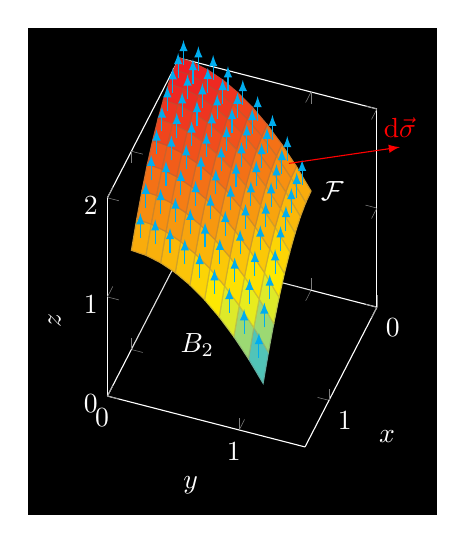
\begin{tikzpicture}[inverted,inverted]
  \pgfmathsetmacro{\px}{0.05};
  \pgfmathsetmacro{\py}{0.85};
  \begin{axis}[inverted,
    width=10cm,
    height=10cm,
    axis equal image,
    view={110}{45},
    xlabel={$x$},
    ylabel={$y$},
    zlabel={$z$},
    xmin=0,xmax=1.5,
    ymin=0,ymax=1.5,
    zmin=0, zmax=2,
    declare function = {
      f(\x,\y) = 2 - \x^2 - \y^2;
      dx(\x,\y) = 2*\x/sqrt(4*\x^2 + 4*\y^2 + 1);
      dy(\x,\y) = 2*\y/sqrt(4*\x^2 + 4*\y^2 + 1);
      dz(\x,\y) = 1/sqrt(4*\x^2 + 4*\y^2 + 1);
    },
    samples=10, samples y=10,
    domain=0:1, domain y=0:1,
    z buffer=sort,
    clip=false,
    ]
    \addplot3[surf,fill opacity=0.2,shader=flat,draw=white,draw opacity=0,colormap/blackwhite] (x,y,0);
    \addplot3[surf,colormap/hot] (x,y,{f(x,y)});
    % vector field
    \addplot3[blue,
      quiver = {
        u = {0},
        v = {0},
        w = {1},
        scale arrows = 0.25,
        every arrow/.append style={-latex},
      },
      samples=9, samples y=9,
      domain = 0.05:0.95,
      domain y = 0.05:0.95,
    ] (x,y,{f(x,y)});
    % surface element
    \draw[->,red] (axis cs: {\px},{\py},{f(\px,\py)}) -- ++ (axis direction cs: {dx(\px,\py)},{dy(\px,\py)},{dz(\px,\py)}) node[above] { $\dd{\vec{\sigma}}$ };
    % labels
    \node[above] at (axis cs: 1,0.5,0) { $B_2$ };
    \node[right] at (axis cs: 0,1,{f(0,1)}) { $\mathcal{F}$ };
  \end{axis}
\end{tikzpicture}
\end{document}
